\subsection{EVL+STrace}
\label{sec:EVLPlusSTrace}

\NOTE{\emph{Solution expert:} Leila , \emph{Interviewer:} Thomas}

\NOTE{Preliminary text by Bernhard (by mistake)}

\NOTE{TODO:  Integrate here as an overview (taken from previous Section 5)}

%\emph{EVL+STrace} \cite{IST2018-Samimi} is based on EMF and the Epsilon framework \cite{epsilon}. A transformation definition is composed of a trace metamodel, which depends on the source and target metamodels, a set of query and update operations defined in EOL, the Epsilon Object Language, and a set of constraints written in EVL, the Epsilon Validation Language. Each constraint is directed, checks for an inconsistency between one of the participating models and the trace model, and repairs this inconsistency by updating both the trace model and the opposite model. Thus, the consistency relation between source and target models is defined by unidirectional checks, and consistency restoration is defined procedurally by the fix parts of the constraints. EVL+STrace supports synchronization between source and target models on demand, making use of a persistently stored trace model. Neither s- nor o-deltas are required. Synchronization is performed interactively by propagating changes in both directions. Automatic synchronization is possible, but requires (mechanical) rewriting of EVL constraints. 

%The bx tool \emph{EVL+STrace} \cite{IST2018-Samimi} supports the synchronization of models on demand (no live synchronization) with the help of a persistently stored \emph{trace model} which stores links connecting source model elements and target model elements. The synchronizer receives the source model, the target model, and the trace model as inputs. After consistency has been established by a previous run of the synchronizer, both source and target models may have been modified. The synchronizer detects inconsistencies between the source model and the trace model, as well as between the trace model and the target model. Consistency is restored by propagating changes in both directions. Consistency restoration is performed interactively: The user is informed about consistency violations and is offered corresponding consistency repair actions. A repair action is performed only when it has been launched explicitly by the user.



The bx tool \emph{EVL+STrace} \cite{IST2018-Samimi} is based on EMF as well as the \emph{Epsilon} framework \cite{epsilon}, which provides tool support for a variety of DSLs for model transformation. In EVL+STrace, a transformation definition consists of a trace metamodel, EOL operations, and EVL constraints (figure~\ref{fig:evlartefacts}). The \emph{trace metamodel} defines domain-specific types of links and link ends. Essentially, the trace metamodel is designed in such a way that a trace model contains copies of all relevant elements of source and target models, as well as links connecting these elements. By means of a rich trace model, it is possible to detect any category of changes to the participating models, including creation and deletion of objects and links, as well as modification of attribute values. The behavior of the synchronizer is defined by \emph{EOL operations}, i.e., operations for queries and updates written in the Epsilon Object Language, and \emph{EVL constraints}, i.e., checks augmented with repair actions written in the Epsilon Validation Language. Each constraint is directed and checks an inconsistency between the trace model and one of the participating models which is caused by a change to this model. The corresponding repair action propagates this change to the trace model and the opposite model.

\begin{figure}[tb!]
	\centering
	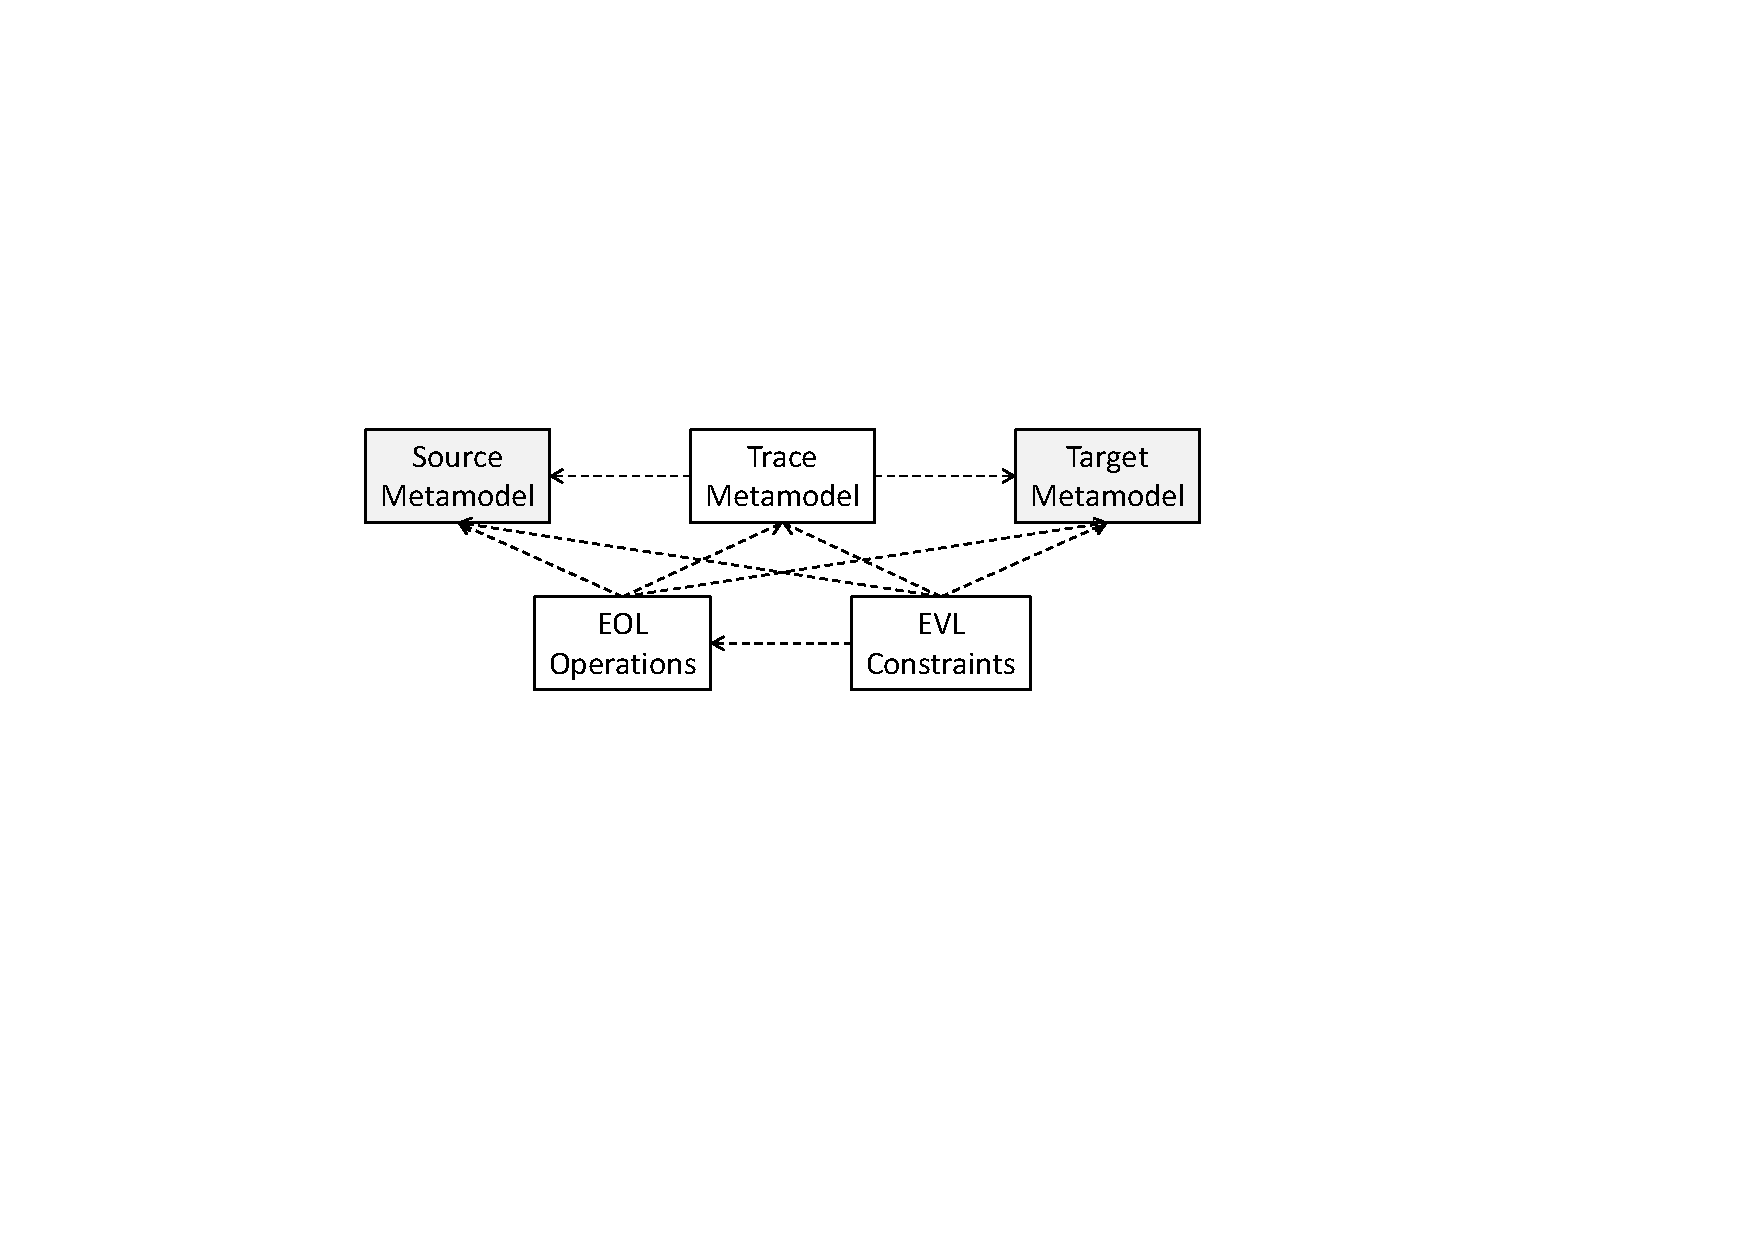
\includegraphics[width=0.8\columnwidth]{diagrams/solutions/EVLPlusSTraceArtefacts}
	\caption{Model artefacts and their dependencies in EVLPlusSTrace}
	\label{fig:evlartefacts}
\end{figure}

%The artefacts making up the transformation definition may be generated partially from a \emph{weaving model}, which essentially includes the trace metamodel, augmented with behavioral properties being specified either by means of parameter values or by code fragments. The generator may create the trace metamodel completely, as well as large parts of EOL operations and EVL constraints, both of which may have to be refined and extended by the transformation developer. In this way, the transformation developer may save the effort of writing routine code for operations and constraints.

\begin{figure*}[tb!]
	\centering
	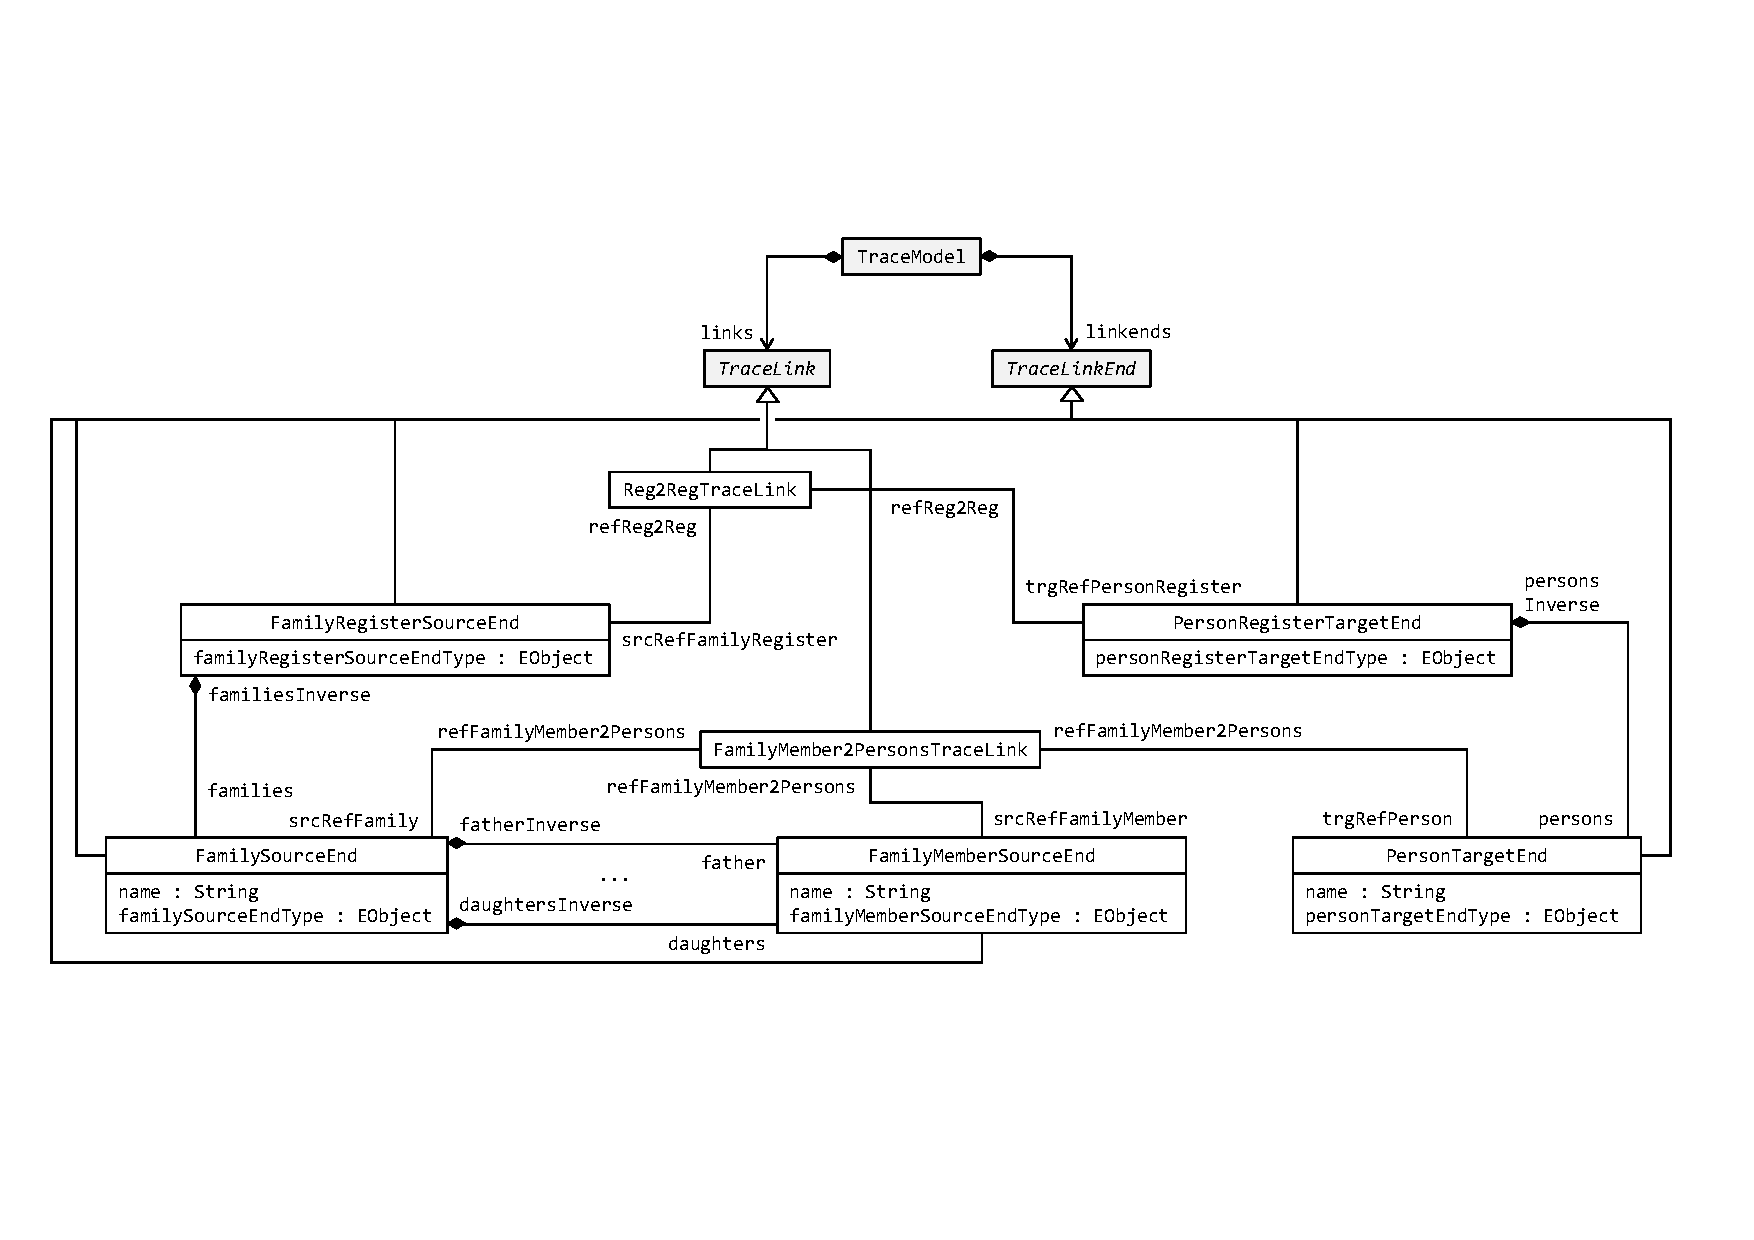
\includegraphics[width=\textwidth]{diagrams/solutions/EVLPlusSTraceMetamodel}
	\caption{Trace metamodel for Families to Persons (without multiplicities)}
	\label{fig:evltracemetamodel}
\end{figure*}

\subsubsection{Classification}
\label{sec:ClassificationEVL}

EVL+STrace provides for \emph{restoration-based} synchronization: it takes the current states of the source and the target model and restores consistency. With respect to horizontal and vertical inputs, EVL+STrace is classified as \emph{initial-diag-based} and realizes the tool architecture displayed in figure~\ref{fig:initialDiagBased} on the left-hand side. 

Similarly to eMoflon, EVL+STrace provides for \emph{stability}, but not for hippocraticness: If an update has been performed which preserves consistency, all constraints will still be satisfied, and no repair action will be performed. However, \emph{correctness} is not guaranteed: Repair actions are specified in a procedural way and may fail to restore consistency.   

%EVL+STrace does not guarantee well-behavedness a priori, i.e., the transformation developer may fail to write a transformation definition which satisfies any of the bx laws mentioned earlier. However, the underlying approach is designed to support the development of \emph{correct} and \emph{hippocratic} transformations: Each constraint may be defined in a declarative way, and a corresponding repair action may be provided such that consistency is reestablished. In this way, correctness may be ensured. Furthermore, since repair actions are guarded by consistency violations, transformations should be hippocratic if no consistency violation occurs.

In EVL+STrace, the \emph{consistency relation} is defined \emph{explicitly} through \emph{constraints}. The overall consistency relation is composed of two sets of directed constraints; the transformation developer is responsible for the mutual consistency of forward and backward constraints. 

EVL+Strace supports \emph{concurrent synchronization} after changes have been applied to both participating models. Directed synchronization is included as a special case: If only one of the participating models has been modified, constraints may be violated only between this model and the trace model. Synchronization is performed \emph{on demand} and \emph{interactively}: Each constraint violation is reported to the user, who has to confirm (or reject) the respective repair action, which is programmed (\emph{explicit control}). Automatic synchronization is possible, but requires rewriting of EVL constraints (see below).

  



\subsubsection{Benchmark solution with EVL+STrace}
\label{sec:solutionEVL}

%EVL+STrace participated in the Families to Persons benchmark at TTC 2017 \cite{Samimi-Dehkordi2017}. The synchronization concept underlying the Benchmarx framework differs from the approach implemented in EVL+STrace in two respects:
%
%\begin{enumerate}
%	\item The synchronization dialogues of the Benchmarx framework assume \emph{alternating changes}: Either an edit on the source model is propagated to the target model, which has not been modified concurrently, or propagation is performed in the opposite direction under analogous assumptions. In contrast, EVL+STrace allows for \emph{concurrent changes}.
%	\item The Benchmarx framework assumes \emph{fully automatic change propagation} without any user interactions (which facilitates testing). In contrast, EVL+STrace supports \emph{fully interactive change propagation}.
%\end{enumerate}
%
%The first issue does not require special attention since EVL+STrace supports the more general case of concurrent changes; however, EVL+STrace will perform redundant checks (for changes on a model which is known to be unmodified) at runtime. We will deal with the second issue (automatic change propagation) at the end of this subsection. 


The following description is based on the solution in EVL+STrace submitted to TTC 2017 \cite{Samimi-Dehkordi2017}.
Figure~\ref{fig:evltracemetamodel} displays the \emph{trace metamodel} for the Families to Persons benchmark. Specific types of trace links and trace link ends are defined by subclassing built-in abstract superclasses \code{TraceLink} and \code{TraceLinkEnd}, respectively. Each \emph{trace link} references a set of trace link ends, which may be considered proxies of source or target model objects. \emph{Trace link ends} store links to source or target model objects with the help of attributes of type \code{EObject}. In addition, trace link ends may store attribute values and may be connected by links. In this way, the trace model may shadow the relevant parts of the source and target models. In the case of the Families to Persons benchmark, the trace metamodel defines two types of trace links for relating family and person registers as well as for relating family members along with their families with persons.


 
\lstdefinelanguage{evl}{
	morekeywords = {context,constraint,guard,not,self,and,check,message,fix,title,do,var,if,else,delete},
	morecomment=[l]{//},
	morecomment=[s]{/*}{*/}
}


\begin{lstlisting}[label={lst:evl}, float=htb!, language=evl, caption={Example of an EVL constraint}]
context Source!FamilyMember{
  constraint isNewMale{
    guard: self.isMale()
    check: not self.isNew()
    message:self+' is a new inserted element 
      in the source model'
    fix{
      title:'Insert its corresponding elements 
        in the trace and target models'
      do {
        var familyMemberSourceEnd 
          = addFamilyMemberSourceEnd(self);
        var family;
        if(self.isFather()) 
          family = self.fatherInverse;
        else 
          family = self.sonsInverse;
        family.satisfies("isNew");
        var familySourceEnd 
          = family.getTraceLinkEnd(); 
        if(self.isFather()) 
          familyMemberSourceEnd
            .setFatherInverse(familySourceEnd);			
        else 
          familyMemberSourceEnd
            .setSonsInverse(familySourceEnd);			
        var person = insertMale(family,self);
        var personTargetEnd 
          = addPersonTargetEnd(person);
        addFamilyMember2PersonsTraceLink(
          familySourceEnd, 
          familyMemberSourceEnd, 
          personTargetEnd);
        copySrc2Trg();
      }
    }
  }
}
\end{lstlisting}

% This is the original code. The code above has been restricted to role changes only. It is not
% clear how the move to another family is handled. The guard of the constraint (stay in the same
% family) excludes a move. Then, the last operand of the check can be eliminated.
%\begin{lstlisting}[label={lst:evl}, float=*t, language=evl, caption={Example of an EVL constraint}]
%context Families2Persons!FamilyMemberSourceEnd{
%    guard: not self.isRemoved() and not self.refFamilyMember2Persons.endTypeIsRemoved()	
%    constraint familyMemberRoleIsRelocated{
%        guard: not self.getEndType().getFamily().isNew() and
%        self.getEndType().getFamily().getTraceLinkEnd()= self.getFamily()
%    check: not ((self.fatherInverse.isDefined() and not self.getEndType().fatherInverse.isDefined())
%        or (self.motherInverse.isDefined() and not self.getEndType().motherInverse.isDefined())
%        or (self.sonsInverse.isDefined() and not self.getEndType().sonsInverse.isDefined())
%        or (self.daughtersInverse.isDefined() and not self.getEndType().daughtersInverse.isDefined())
%        or (self.getEndType().getFamily().getTraceLinkEnd()<> self.getFamily()))		
%        message: self+' role is changed or\n'+self+' family ='+self.getFamily()+ 
%            'is changed to '+self.getEndType().getFamily()
%    fix{
%        title: 'Propagate the relocation for '+self
%    do{
%        var family= self.getEndType().getFamily();
%        var person;
%        if((self.fatherInverse.isDefined() or self.sonsInverse.isDefined()) and
%            self.getEndType().isFemale()){
%            person =insertFemale(family,self.getEndType());
%            person.birthday = self.refFamilyMember2Persons.trgRefPerson.getEndType().birthday;
%            var personTargetEnd = addPersonTargetEnd(person);
%            delete self.refFamilyMember2Persons.trgRefPerson.getEndType();
%            delete self.refFamilyMember2Persons.trgRefPerson;
%            self.refFamilyMember2Persons.trgRefPerson = personTargetEnd;
%        }
%        else 
%            if((self.motherInverse.isDefined() or self.daughtersInverse.isDefined()) and
%                 self.getEndType().isMale()){
%                        person = insertMale(family,self.getEndType());
%                        person.birthday = self.refFamilyMember2Persons.trgRefPerson.getEndType().birthday;
%                        var personTargetEnd = addPersonTargetEnd(person);				
%                        delete self.refFamilyMember2Persons.trgRefPerson.getEndType();
%                        delete self.refFamilyMember2Persons.trgRefPerson;
%                        self.refFamilyMember2Persons.trgRefPerson = personTargetEnd;}
%                        self.refFamilyMember2Persons.srcRefFamily = family.getTraceLinkEnd();	
%                        copySrc2Trg();
%
%}
%}
%}
%}
%...
%}
%\end{lstlisting}

Listing~\ref{lst:evl} gives an example of an \emph{EVL} constraint along with its repair action. The constraint refers to family members in the families models (line~1). As indicated by the name of the constraint (line~2), it handles the creation of a new male member. Its guard (line~3) ensures that it may be applied only to male family members. The check (line~4) defines that the member must not be new, i.e., there must be a corresponding person in the persons model. If this check fails, a meaningful message (line~5) is created which is displayed at the user interface. The fix (line~6) has a title (line~7) which explains the repair action to the user, as well as a \code{do} part (starting at line~8) which defines all operations to restore consistency in a procedural way. Please note that these operations refer both to the persons model and the trace model.

%Listing~\ref{lst:evl} gives a (slightly simplified) example of an \emph{EVL} constraint which deals with the relocation of a family member role. The \emph{context} in line~1 defines the set of objects on which the constraints inside the context declaration have to be evaluated (family member source ends in the trace model). The \emph{guard} in line~2 is shared by all constraints inside the context declaration and ensures that the member has not been removed (otherwise, the constraints are not applicable). The \emph{constraint declaration} starting in line~3 deals with the relocation of the role of a family member. The \emph{check} in lines~4--8 specifies the condition which has to be maintained: The family member must not have changed its role. The condition is checked by comparing links in the trace model against links in the families model. If a violation of this condition is detected (i.e., the role has changed), the \emph{message} in line~8 is used to inform the user about the violation. The proposed \emph{fix} is specified starting from line~9. The \emph{title} in line~10 is used to describe the fix to the user. The actual fix is contained in the \emph{do block} starting in line~11: The old person object is replaced with a new person object of the opposite gender to which the birthday of the old person object is copied.

The Families to Persons benchmark deviates from the synchronization scenario targeted by EVL+STrace in two respects. First, the benchmark comprises only alternating rather than concurrent changes, i.e., only one model is changed, and the opposite model is updated to restore consistency. Second, the test suite is executed automatically, without any user interaction.

Since EVL+STrace supports a more general type of synchronization than demanded by the benchmark, it may also handle alternating changes as it stands. For automatic synchronization, the constraint definitions have to be modified by moving the \code{do} part into the \code{check} part and eliminating the \code{message} and the \code{fix} part. These mechanical transformations were applied throughout the EVL code to execute the Families to Persons benchmark without user interaction. 